\documentclass{hfutpaper}
\usepackage[urlcolor=blue]{hyperref}
\usepackage{threeparttable}
\usepackage{setspace}
\usepackage{titlesec}
\usepackage{float}
\usepackage{verbatim}
\newcommand{\upcite}[1]{\textsuperscript{\textsuperscript{\cite{#1}}}}
\usepackage{fancyhdr}
\titleformat{\section}{\large \heiti}{\chinese{section}、}{0em}{}
\begin{document}
\begin{center}
\LARGE
  \textbf{对于量子计算和量子计算机的初步了解}\\
  \vspace{0.2em}
  \large
    崔博 \ \ \ 55180520 \\ %姓名,学号,班级
  \end{center}
\rule[0.1\baselineskip]{\textwidth}{0.5pt}
\\
\textbf{摘 \ 要}\\
\large
量子计算机可以比传统计算机更有效地处理大量复杂地数据集。他们利用量子力学的基本原理来加速解决复杂计算的过程。这些计算通常包含看似无限数量的变量,潜在的应用,跨越了从基因组学到金融的各个行业。
\\
\textbf{关键词}:量子\quad 计算\quad 应用\\
\rule[0.1\baselineskip]{\textwidth}{0.5pt}
\section{引言}
1965年,英特尔联合创始人戈登·摩尔(Gordon Moore)观察到,微芯片上每平方英寸的晶体管数量每年会翻一番,同时成本却减少了一半(自1958年发明晶体管以来)。 这个观察结果被称为摩尔定律。

摩尔定律意义重大,因为它意味着随着时间的推移,计算机会变得越来越小、计算能力越来越强、计算速度越来越快。

然而,摩尔定律正在慢下来(有些人说停止了) ,传统计算机没有以过去那样的速度进步。

在2020年代的某个时候,如果我们想继续从计算能力的指数增长中获益,我们必须找到一种完全不同的信息处理方式。

进入量子计算。
\section{近年进展}
中国科学技术大学潘建伟、朱晓波团队,联合浙江大学王浩华团队,利用超导电路实现了10量子位(qubit )的量子纠缠,突破了之前9量子位的记录,向实现大规模量子计算迈出重要一步。相关成果于2017年11月3日发表在Physical Review
Letters上。

2017年11月11日,IBM宣布取得重大进展,20量子位的量子计算机问世,并构建了50量子位的量子计算机原理样机。20量子位的量子计算机的相干时间较之前翻倍,平均相干时间由50微秒提升到90微秒,而且其设计具有可扩展性;50量子位的量
子计算机也有相似表现。IBM团队展望:“在即将到来的一年,量子计算将会为化学、最优化和机器学习打开新的大门。”

2017年11月20日,日本宣布将推出首台量子计算机的原型机。日本国家情报学研究所( NationalInstitute of Informatics, NII )、日本电报电话公司(Nippon Telegraph\&Telephone,NTT)以及东京大学的研究人员宣称.正在研制一款可以承载“量子神经网络”技术的云端系统,此系统可以解决城市交通堵塞问题,优化人群密集地带手机与基站之间的联系,通过对各种化学物质进行模拟来开发出新药物。理论上此系统的计算速度是传统超级计算机的100倍,能耗却只有其1/l0,2020年3月将此系统商业化。

哈佛大学卢金(M. Lukin),格雷纳(M. Greiner)与麻省理工学院武莱蒂奇( V. Vuletic)通过激光捕获超冷铆原子,并将冷原子以特定顺序排列,开发出一种51量子位的量子模拟器,可以实现特定的量子计算。该系统有效结合了大尺度系统与高维度的量子相干性,是目前最大的量子计算系统之一。相关成果于2017年11月30日发表在Nature上。马里兰大学联合量子研究所(Joint Quantum  Institute)以及美国国家标准与技术研究院(National Institute of Standardsand Technology, NIST)研制出一种53量子位的量子模拟器,用于探索复杂的量子多体系统,观测到多体动力学相变。相关成果于2017年11月30日发表在Nature上。新南威尔士大学研究团队通过重新构思、设计硅微处理器,提出一种基于现有半导体元件、当前工业水平下可量产的量子计算芯片。相关成果于2017年12月15日在线发表于Nature Communications。

目前,最先进的量子计算芯片,由总部位于伯克利的初创公司 Rigetti Computing开发,可以使用多达19个量子比特,该公司宣布,到2019年底制造一个128个量子比特的芯片。
\iffalse
\begin{table}[H]
	\caption{表格}
	\centering
	\begin{tabular}{cccccccc}
		\toprule[1.5pt]
		年份  & 2006&2007&2008&2009&2010 & 2011 & 2012 \\
		\midrule
		A&57.95&58.187&59.1&59.652&60.22&61.072&61.418 \\
		B &55.7957 &58.3199&58.8548&59.9983&60.3769 &60.9841 &61.7716 \\		
		C&2.1543&0.1329&0.2452&0.3463&0.1569&0.0879&0.3536 \\		
		D&0.0372 &0.0023&0.0041&0.0058&0.0026&0.0014&0.0058 \\
		\bottomrule[1.5pt]
		\label{tab1}
	\end{tabular}
\end{table}
\fi
\section{量子比特}
量子计算机可以提供巨大的效率优势,来解决困扰当今计算机的某些类型的计算的问题,即使摩尔定律将无限期地继续下去,量子计算机也将继续困扰它们。

首先,想象一下电话簿,然后想象你有一个特定的号码可以在电话簿中查找。传统的计算机会搜索电话簿的每一行,直到找到并返回匹配结果。
理论上,量子计算机可以即时搜索整个电话簿,同时评估每一行,并比经典计算机更快地返回结果。
这些问题需要变量和解决方案的最佳组合,通常被称为优化问题。它们是世界上最复杂的问题,有可能改变游戏规则。

量子计算可以帮助将所有变量考虑在内,以帮助我们最有效地规划大规模项目。
各个行业都面临优化问题,包括软件设计、物流、金融、网络搜索、基因组学等等。
虽然这些行业中最棘手的优化问题难倒了经典计算机,但量子机器非常适合解决这些问题。

量子计算机与传统计算机的不同之处在于,传统计算机的改进主要依赖于构成晶体管和微芯片的材料的进步。
量子计算机不使用晶体管(或经典比特)。相反,它们使用使用量子比特。
量子比特是量子计算机中处理信息的基本单位。
\begin{figure}[H]%H表示图强制在下面,想设置浮动环境用htp
	\centering  %插入的图片居中表示
	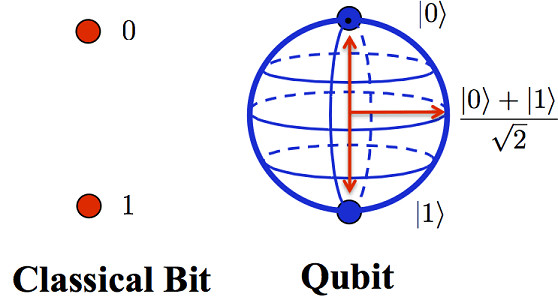
\includegraphics[scale=0.5]{qu}  %插入的图,包括JPG,PNG,PDF,EPS等,放在源文件目录下
	\caption{量子比特}  %图片的名称
	\label{fig1}
\end{figure}
量子位可以是0到1之间的任意值,或者同时具有这两个值的属性。现在,执行计算的可能性要多得多。%\upcite{bib:two}

在量子系统中,我们也可以寻找天然的双态系统来实现这两种可区分的状态。比如自旋系统,一个电子的自旋有上下之分,我们可以把测量到“上”定义为1,而测量到“下”则定义为0,这就构成了一个量子比特。神奇的地方在于,量子力学告诉我们一个量子比特可以制备在两个逻辑态0和1的相干叠加态上,换句话讲,它可以同时存储0和1。考虑一个有N个物理比特的存储器:若它是经典存储器,则它只能存储$2^N$可能数据当中的任个;若它是量子存储器,则可以同时存储$2^N$数,这意味着随着N的增加,其存储信息的能力将指数上升。例如,一个250量子比特的存储器(由250个原子构成)可能存储的数量达$2^250$,比目前己知的宇宙中全部原子的数目还要多。

由于数学操作可以同时针对存储器中全部的数据进行,因此量子计算机在实施一次的运算中可以同时对$2^N$输入数进行数学运算。其效果相当于经典计算机要重复实施$2^N$次操作,或者采用$2^N$不同处理器实行并行操作。可见,量子计算机可以节省大量的运算资源(如时间、记忆单元等)。
\section{量子计算主要类型}
量子计算主要有三种类型。 每种类型的不同之处在于所需的处理能力(量子比特)的数量,可能的应用数量,以及实现商业可行性所需的时间。

一、量子退火

量子退火适用于一系列的工业问题。 例如,2015年,以开发军用和商用飞机而闻名的全球航空航天和国防公司空中客车在其英国纽波特工厂建立了一个量子计算部门。
这家公司正在探索将量子退火用于数字建模和材料科学。

\begin{figure}[H]%H表示图强制在下面,想设置浮动环境用htp
	\centering  %插入的图片居中表示
	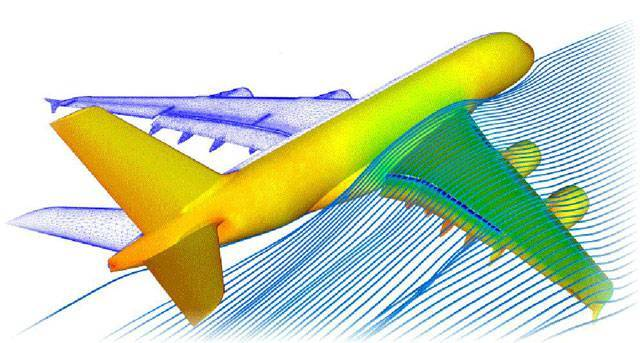
\includegraphics[scale=0.5]{anneal}  %插入的图,包括JPG,PNG,PDF,EPS等,放在源文件目录下
	\caption{飞机机翼的建模}  %图片的名称
	\label{fig1}
\end{figure}

目前,工程师们需要花费数年时间来模拟飞机机翼上空的空气流动过程,而量子计算机只需要几个小时来模拟机翼上空以各种角度和速度流动的每一个空气原子,就可以确定最佳或最有效的机翼设计。

量子退火是量子计算中功能最弱、应用范围最窄的一种形式。
事实上,专家们一致认为,今天的超级计算机可以解决一些优化问题,就像今天的量子退火计算机一样。

二、量子模拟

量子模拟探索量子物理学中超出传统计算系统能力的特定问题。模拟复杂的量子现象可能是量子计算的重要应用之一。

有一个特别有希望的领域,是模拟化学刺激对大量亚原子粒子的影响,称为量子化学。
特别是,量子模拟器可以用来模拟蛋白质折叠,这是生物化学中最棘手的问题之一。

错误折叠的蛋白质会导致像阿尔茨海默氏症和帕金森氏症这样的疾病,测试新疗法的研究人员必须通过使用随机计算机模型来了解哪些药物会引起每种蛋白质的反应。

据说,如果一种蛋白质要通过顺序取样所有可能的药物诱导效应而找到正确的折叠结构,它需要比宇宙年龄更长的时间才能找到其正确的自然状态。

\begin{figure}[H]%H表示图强制在下面,想设置浮动环境用htp
	\centering  %插入的图片居中表示
	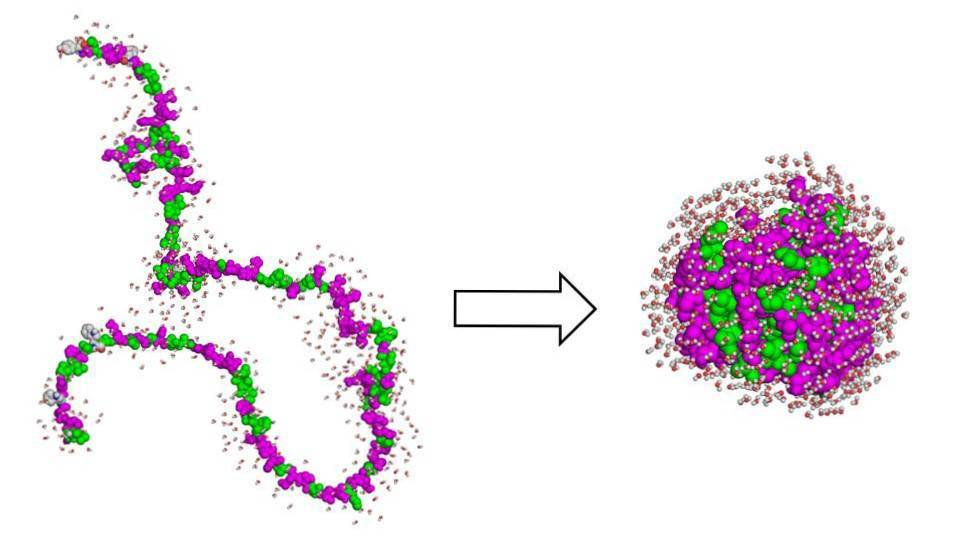
\includegraphics[scale=0.5]{protein}  %插入的图,包括JPG,PNG,PDF,EPS等,放在源文件目录下
	\caption{蛋白质结构折叠示意图}  %图片的名称
	\label{fig1}
\end{figure}

绘制一个真实的蛋白质折叠序列,将是一个重大的科学和医疗保健突破,可以拯救生命。
量子计算机可以帮助计算大量可能的蛋白质折叠序列,以制造更有效的药物。 在未来,量子模拟将通过解释每一种可能的蛋白质-药物组合,使快速设计药物测试成为可能。

三、通用量子计算

\begin{figure}[H]%H表示图强制在下面,想设置浮动环境用htp
	\centering  %插入的图片居中表示
	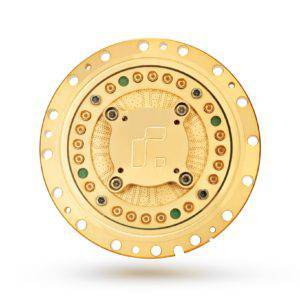
\includegraphics[scale=0.5]{chip}  %插入的图,包括JPG,PNG,PDF,EPS等,放在源文件目录下
	\caption{Rigetti的量子芯片}  %图片的名称
	\label{fig1}
\end{figure}

通用量子计算机是最强大、最通用的,但也是最难制造的。一台真正通用的量子计算机可能会使用超过10万个量子比特,一些人估计会达到100万个量子比特。请记住,今天,我们能做到的最多的量子比特甚至不到128个。

通用量子计算机背后的基本思想是,你可以指导机器进行任何复杂的计算,并快速得到解决方案。这包括求解上述的退火方程,模拟量子现象,等等。
多年来,研究人员一直在设计只能在通用量子计算机上使用的算法。最著名的算法是Shor的分解数字算法(用于高级代码破解) ,以及Grover的快速搜索非结构化和海量数据集的算法(用于高级互联网搜索等)。

至少有50种其他独特的算法已经开发出来,可以在通用量子计算机上运行。
在遥远的未来,通用量子计算机可以彻底改变人工智能领域。量子人工智能可以实现比传统计算机更快的机器学习。

最近的研究已经产生了可以作为量子机器学习基石的算法,但是对于我们来说,完全实现量子人工智能的硬件和软件仍然像一般的量子计算机本身一样难以捉摸。

\section{量子计算类型---Shor和Grower算法}

为开拓出量子计算机巨大的并行处理能力,还必须要寻找适用于这种量子计算的有效算法。Shor于1994年发现了第一个量子算法,它可以有效地用来进行大数因子分解。目前,广泛用于电子银行、网络等领域的公开密钥体系“RSA",其安全性的前提便是“大数因子难以用经典计算机分解”。现有计算机对个长度为n的大数做因子分解,其运算时间以$2^{n/2}$
的指数增长。迄今,在实验中被分解的最大数为129位,1994年在世界范围内同时使1600个工作站花8个月时间才成功地完成这个分解。用同样计算功能来分解250位的数要用80万年,而对于1000位的数,则要用$10^{25}$年。采用Shor算法的量子计算机所需时间仅以$n^{2(lgn)(lglgn)}$增长,大大减少了时间复杂度,可以在几分之一秒内实现对1000位数的因子分解。可见,Shor量子算法将这类“难解”问题(NP问题)变成“易解”问题(P问题)。这意味着在量子计算机面前,现有公开密钥RSA体系将成为摆设!Shor算法的开创性工作有力地刺激了量子计算机和量子密码术的发展,成为量子信息科学发展的重要里程碑之一。

另一个非常有用的量子算法是1997年Grove提出的搜寻算法,即所谓的量子搜寻算法,也称Grover算法。它专注于解决在N个未分类的客体中寻找出某个特定的个体。通俗地说,它可解决如下问题:要从有着100万个号码的电话本中找出某个指定号码,该电话本是以姓名为顺序编排的。经典方法是一个个找,平均要找50万次,才能以50\%概率找到所要电话号码。而Grover的量子算法每查询一次就可以同时检查所有100万个号码。100万量子比特处于叠加态,量子干涉的效应会使前次的结果影响到下一次的量子操作,这种干涉生成的操作运算重复1000(即$\sqrt{N}$)次后,获得正确答案的概率为50\%。若再多重复操作几次,那么找到所需电话号码的概率接近于
100\%。

\section{量子计算机的物理系统}

我们现在找到了实用性的算法,那么如何在物理上实现量子计算机的硬件呢?科学家们开始的设想是从传统电路的逻辑出发,只要能找到一个易于测量的双态体系,如光子的偏振方向,电子、原子核的自旋方向或原子、离子本身任意两个离散的能级构成的二能级系统,将它们组成大规模的阵列,再通过光、电、磁场等干涉方法组成一系列“量子逻辑门”对其进行操控,就可以构建出初步的量子计算机。

遗憾的是在实际中,原子尺度的粒子很容易受到环境中噪声的干扰,从而失去量子效应(退相干)进而导致量子比特发生错误,因此必须将环境温度控制在一273 K左右(与绝对零度相差不到一度)。另外由于测量引起的“坍塌效应”,我们无法直接读取一个量子位的状态,只能通过测量与其纠缠的其他粒子来推测出它的状态。所以为了纠错和读取,每一个逻辑比特都需要5000-10000个物理L匕特来进行辅助。

目前,备受人们期待能实现量子计算的物理系统有离子阱系统、超导约瑟夫森结系统、金刚石自旋系统、半导体量子点系统以及我国潘建伟教授研发的国际领先的光子系统等。它们各有优缺点,比如:离子阱系统“干净”(相干时间长)且‘精密(量子态制备保真度高),但其所需操控时间长且大规模集成困难;超导量子系统对量子比特和量子逻辑门的操控可达到纳秒(十亿分之一秒)级别,但抗噪声能力不能令人满意。种种诸如此类的困难,使得多年过去人们也只能在实验室内做到数十个量子比特的量子计算原型机。

\section{量子计算的投资者}

随着整个行业领域的利益增加,支持这些公司发展的整体生态系统也在增长。主流风险投资家和大公司已经开始在初创量子计算公司身上下注。

谷歌风投(Google Ventures)和亚马逊等公司都投资了IonQ,这家公司正在开发通用量子计算机,以应对广泛的应用。

这个领域中著名的风投公司包括红杉资本,投资了量子计算硬件公司Quantum Circuits。 安德森·霍罗威茨公司(A16Z)已经投资了Rigetti Computing;Draper Fisher Jurvetson已经参与到了对D-Wave的多轮投资。

2018年2月,随着韩国移动电信运营商SK Telecom加入“游戏”,量子计算在通信安全方面的关注也得到了提升,几个月后,德国的Deutsche Telekom也加入了进来。

这两家电信公司在6500万美元的投资中,购买ID Quantique的多数股权和少数股权。ID Quantique 提供基于量子技术的多协议网络加密,以确保通信安全。

一些世界上最大的公司也在公司内部启动了量子计算项目。

在谷歌量子人工智能实验室中,运行着一台D-Wave的量子计算机。这个实验室位于加利福尼亚州山景城的NASA的Ames研究中心,由NASA和大学空间研究协会主持。

2015年7月,阿里巴巴的阿里云部门和中国科学院在上海建立了一个名为阿里巴巴量子计算实验室的研究机构。 这家实验室研究电子商务和数据中心的量子安全技术。

2019年1月,IBM在CES上推出了第一台商用量子计算机。IBM的Q System One使用20个量子比特,既有传统计算机的组件,也有量子计算机的组件。

这家公司在声明中清楚地表明,商用量子计算机要打败今天的传统计算机还需要时间。

包括惠普、英特尔和微软在内的一系列其他科技公司也在部署量子计算。
一些国防承包商和咨询公司也开始研究量子计算机,包括:Booz Allen Hamilton、Lockheed Martin、Raytheon等等。
除了公司投资,欧盟、美国、澳大利亚和中国也在支持旨在建造量子计算机的项目。

2016年,中国发射了世界上第一颗量子卫星,以寻求更安全的通信。

\section{量子霸权离我们的距离}

量子计算机的优势,在于它能够解决传统计算机实际上无法解决的问题。理想的量子计算机会是一个普遍适用的计算机,并优于传统计算机。

公司和政府都在研发量子计算机,实现量子霸权。例如,2018年3月,谷歌声称其72量子比特芯片比传统机器更快地解决了一个精心挑选的问题。
宣布后不久,阿里巴巴的研究人员宣布他们已经用传统系统解决了同样的问题。这种隔空交流强调了世界上最强大的公司竞相主导量子霸权的真实性。

现在,包括D-Wave Systems、阿里巴巴、IBM和Rigetti Quantum Computing等公司生产的最强大的量子计算机,是一种混合传统和量子的产品。
也就是说,它们提供了一个强大的传统系统的混合体,由令人印象深刻的量子能力推动。

然而,这个行业正在快速发展。 专家们一致认为,到2030年,我们可以看到量子计算机超越传统计算机。
在量子计算实现其潜力之前,必须要克服重大的技术障碍。这将需要开发更稳定的硬件、用于软件开发的商业平台,以及开发用于分配和访问量子计算资源的云计算能力。

\begin{thebibliography}{9}%宽度9
\bibitem{bib:one} 
王晋岚.量子计算最新进展[J].科学,2018,70(01):8.

\bibitem{bib:two} 
李亦超.借用“平行宇宙”的算力——量子计算现状与展望[J].自然杂志,2019,41(05):364-369.

\bibitem{bib:three} 
量子纠缠技术在地质学上应用的可能性[J].张旗,焦守涛,李明超,朱月琴,韩帅,刘学龙,金维浚,陈万峰,刘欣雨.地学前缘.2019(04).

\bibitem{bib:four} 
经典逻辑门与量子逻辑门[J].张登玉,谭咏康.衡阳师范学院学报. 2019(03)

\bibitem{bib:five}
量子信息引论[J].郭光灿.物理.2001(05).

\bibitem{bib:six}
Quantum machine learning.Wittek P.Nature .2017.

\bibitem{bib:seven}
Discrete optimization using Quantum Annealing on sparse Ising models.Bian Z,Chudak F,Israel R,et al.Frontiers in Physics.2014.

\bibitem{bib:eight}
36Kr.一文看懂量子计算:原理、应用、行业现状.https://36kr.com/p/5174475.
\end{thebibliography}
\iffalse
\section*{matlab源程序}
\begin{lstlisting}[language=matlab]
clc;clear;
row = size(A) 
row = size(A,1) 
column = size(A,2) 
[row,column] = size(A) 
\end{lstlisting}
\fi
\end{document} 